
\documentclass[14pt,compress,aspectratio=1610]{beamer}

\usepackage[english]{babel}
\usepackage[english]{isodate}
\isodate
\usepackage{multicol}
\usepackage{tikz}
\usepackage{varwidth}

\usetheme{vertex}

\linespread{1.3}
%\setbeamerfont{itemize/enumerate body}{size=\Large}
%\setbeamerfont{itemize/enumerate subbody}{size=\Large}
%\setbeamerfont{body}{size=\Large}

\title{Particle Clicker}
%\subtitle{A simple, engaging detector game}
\subtitle{ }
\institute{CERN webfest 2014}

\begin{document}

% The title page needs an event display
\maketitle

{
    \setbeamertemplate{navigation symbols}{}
    \begin{frame}[plain]
        \begin{tikzpicture}[remember picture,overlay]
            \node[at=(current page.center)] {
                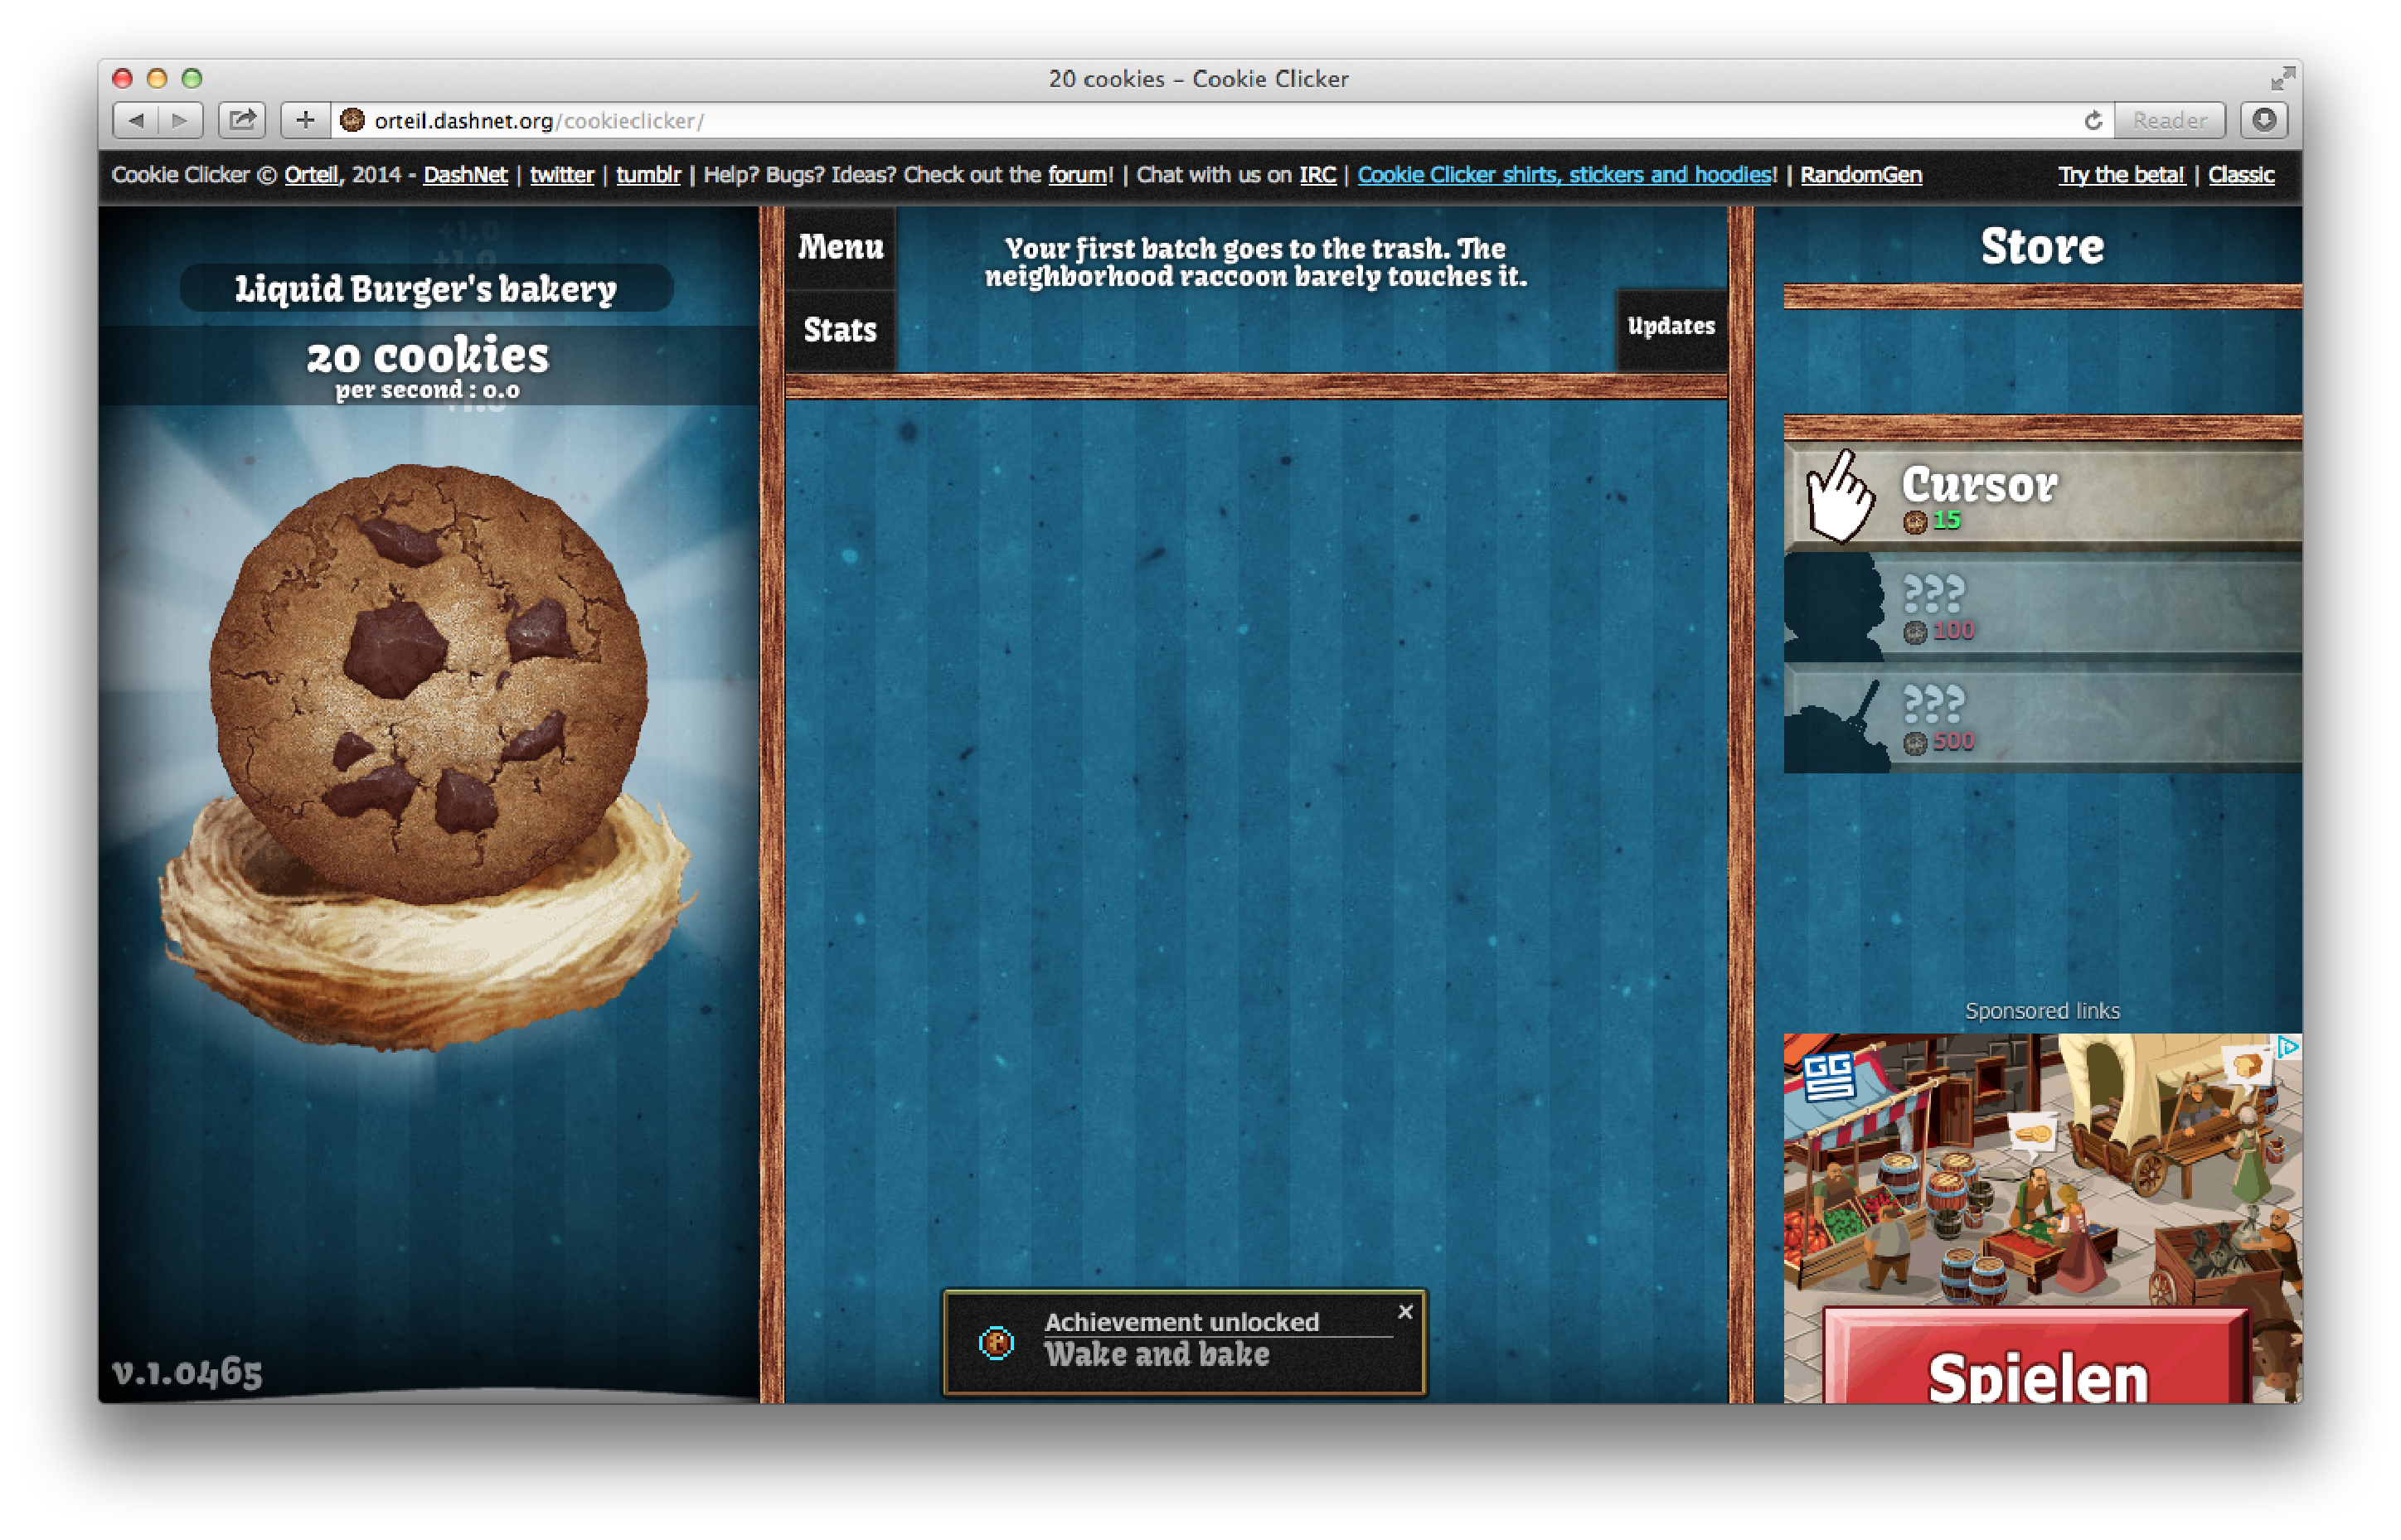
\includegraphics[width=\paperwidth]{figures/cc.pdf}
            };
        \end{tikzpicture}
     \end{frame}
}

{
    \setbeamertemplate{navigation symbols}{}
    \begin{frame}[plain]
        \begin{tikzpicture}[remember picture,overlay]
            \node[at=(current page.center)] {
                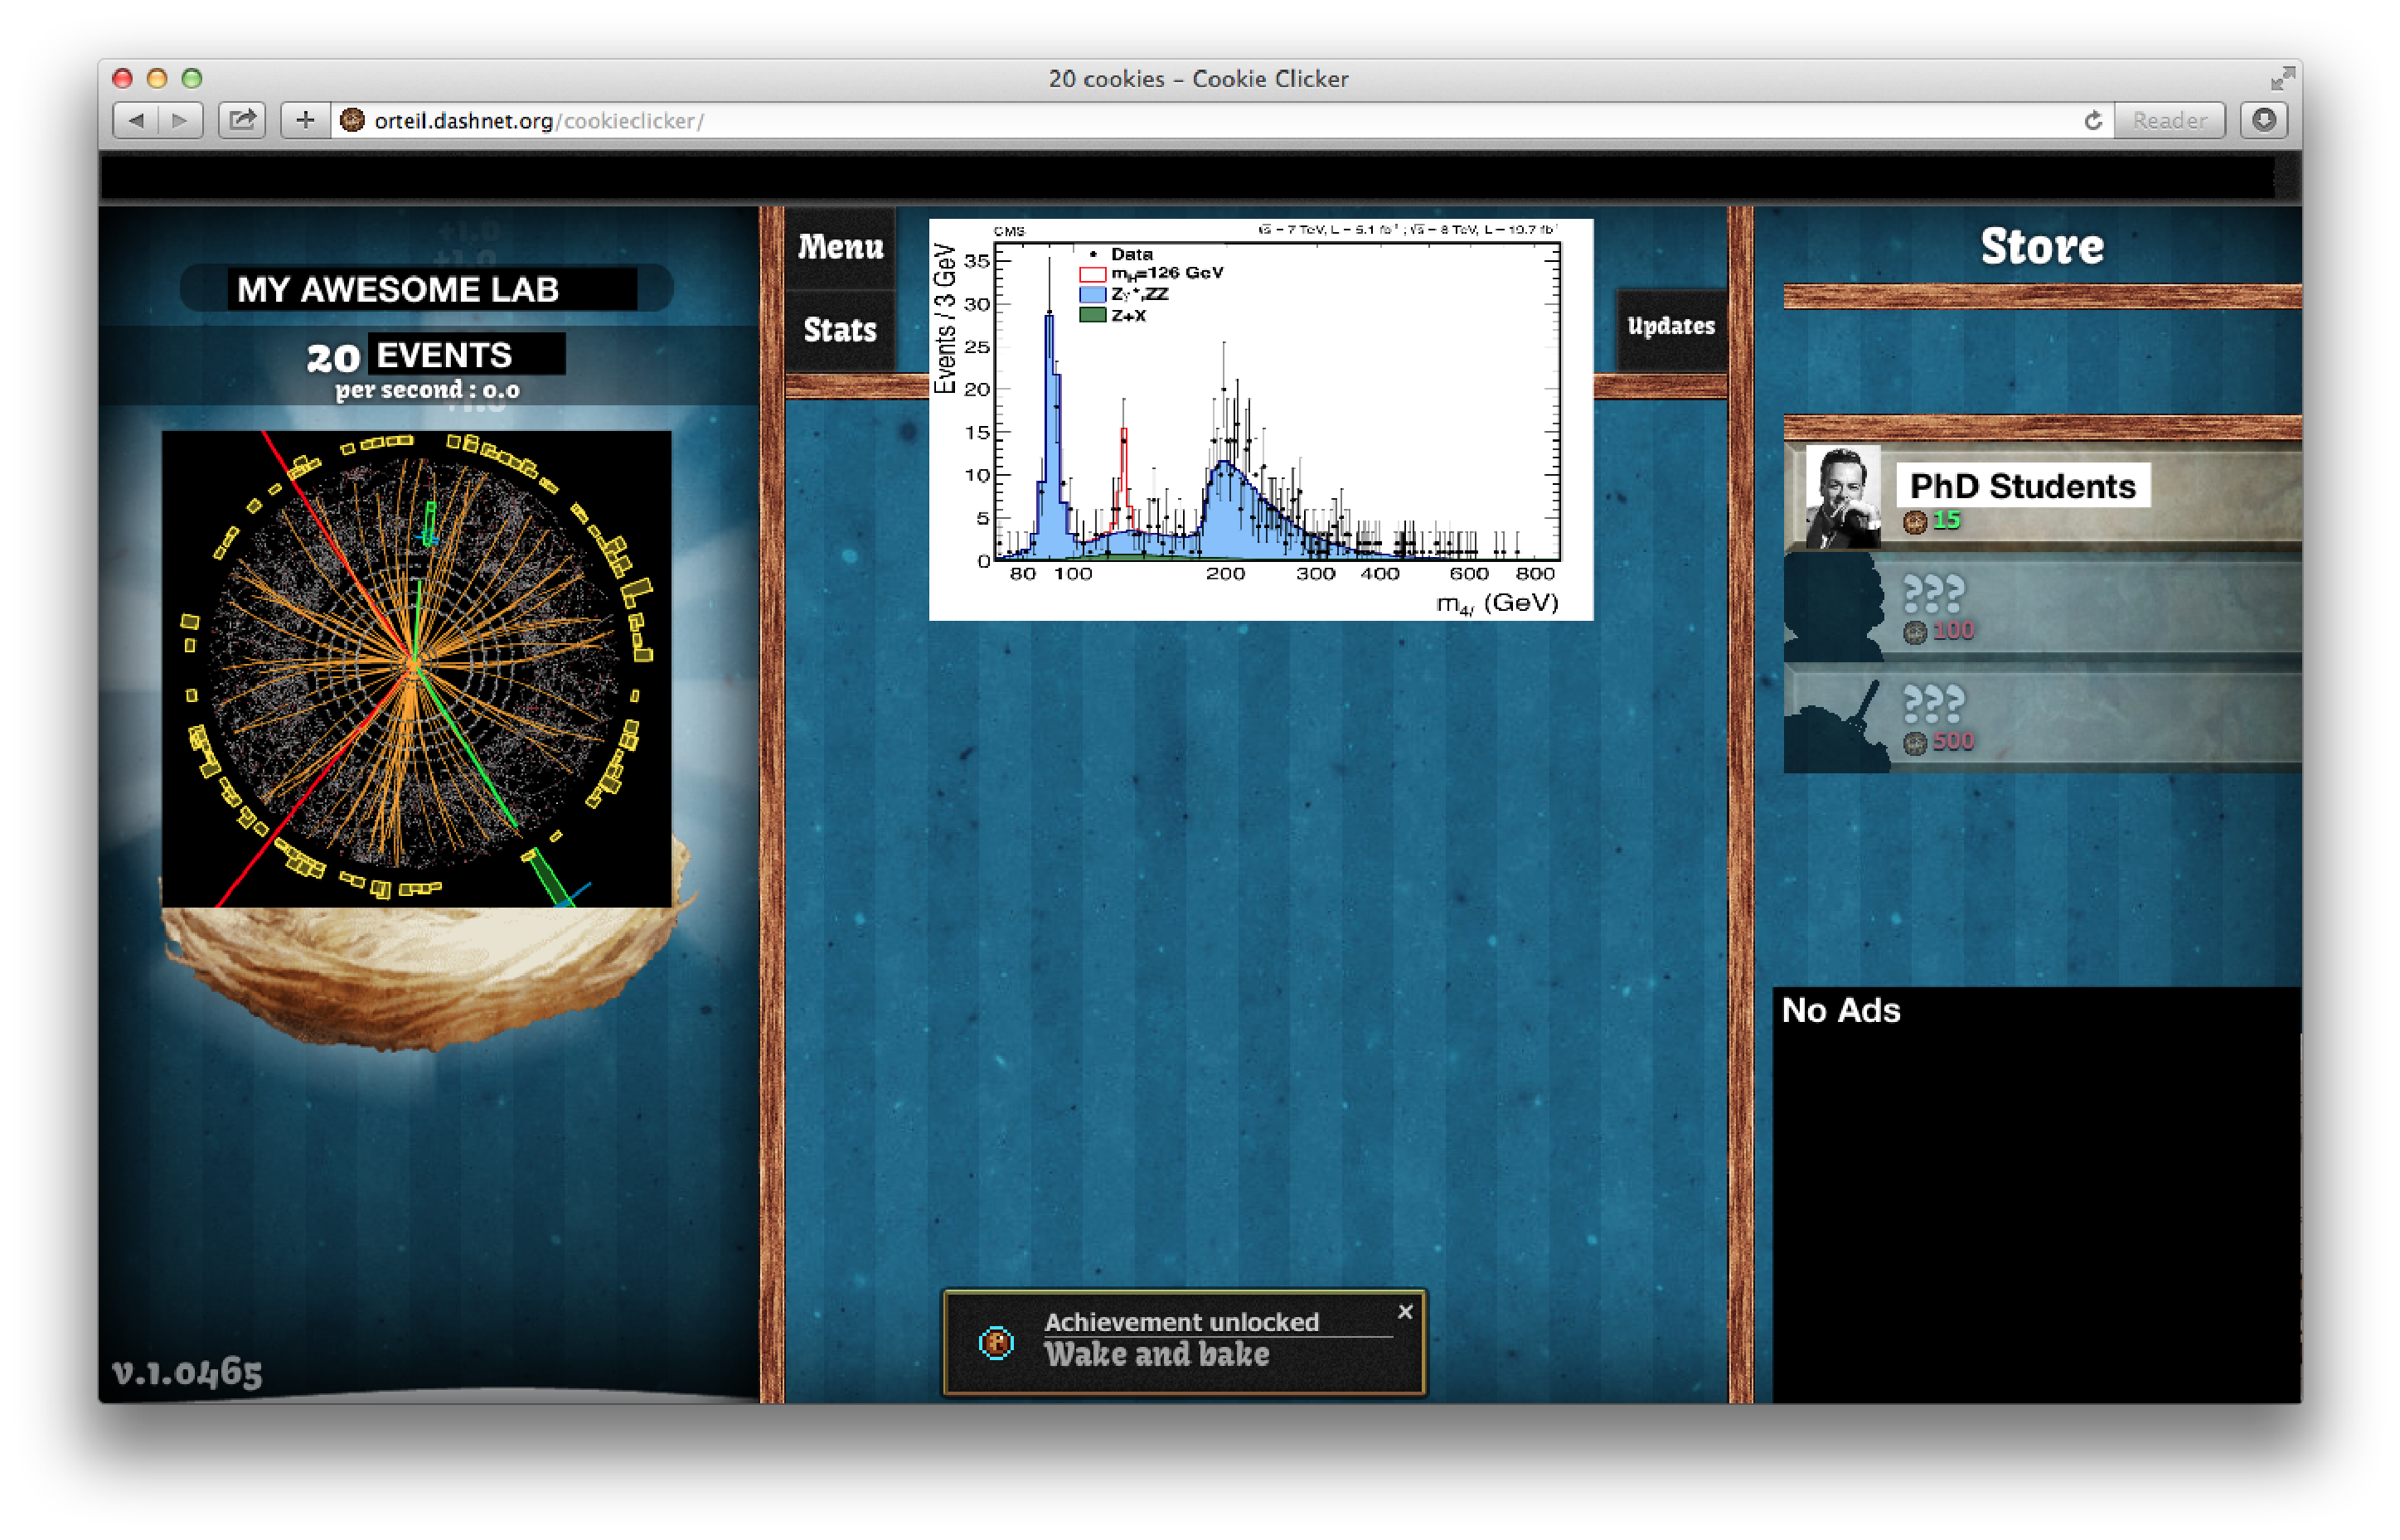
\includegraphics[width=\paperwidth]{figures/pc.pdf}
            };
        \end{tikzpicture}
     \end{frame}
}

\begin{frame}{Goals for the weekend}
  \begin{center}
  \begin{varwidth}{4in}
  \begin{itemize}
    \item Create a working game from scratch
    \begin{itemize}
      \item Single page HTML/Javascript app
    \end{itemize}
    \item Have lots of fun!
  \end{itemize}
  \end{varwidth}
  \end{center}
\end{frame}

\begin{frame}{What are we looking for?}
  Any of the following:

  \begin{center}
  \begin{varwidth}{4in}
  \begin{itemize}
    \item Experience with HTML/Javascript
    \item 2d design skills
    \item Desire to test and improve the gameplay
  \end{itemize}
  \end{varwidth}
  \end{center}

  \centering
  
\includegraphics[width=0.8in]{figures/git.png}
  
\includegraphics[width=1in]{figures/html5.png}
  
\includegraphics[width=0.73in]{figures/js.png}
\end{frame}

\begin{frame}[plain]
  \centering
  \linespread{1}
  \huge
  \vspace{1em}
  Have a smashing weekend!
  \vspace{0.5em}

  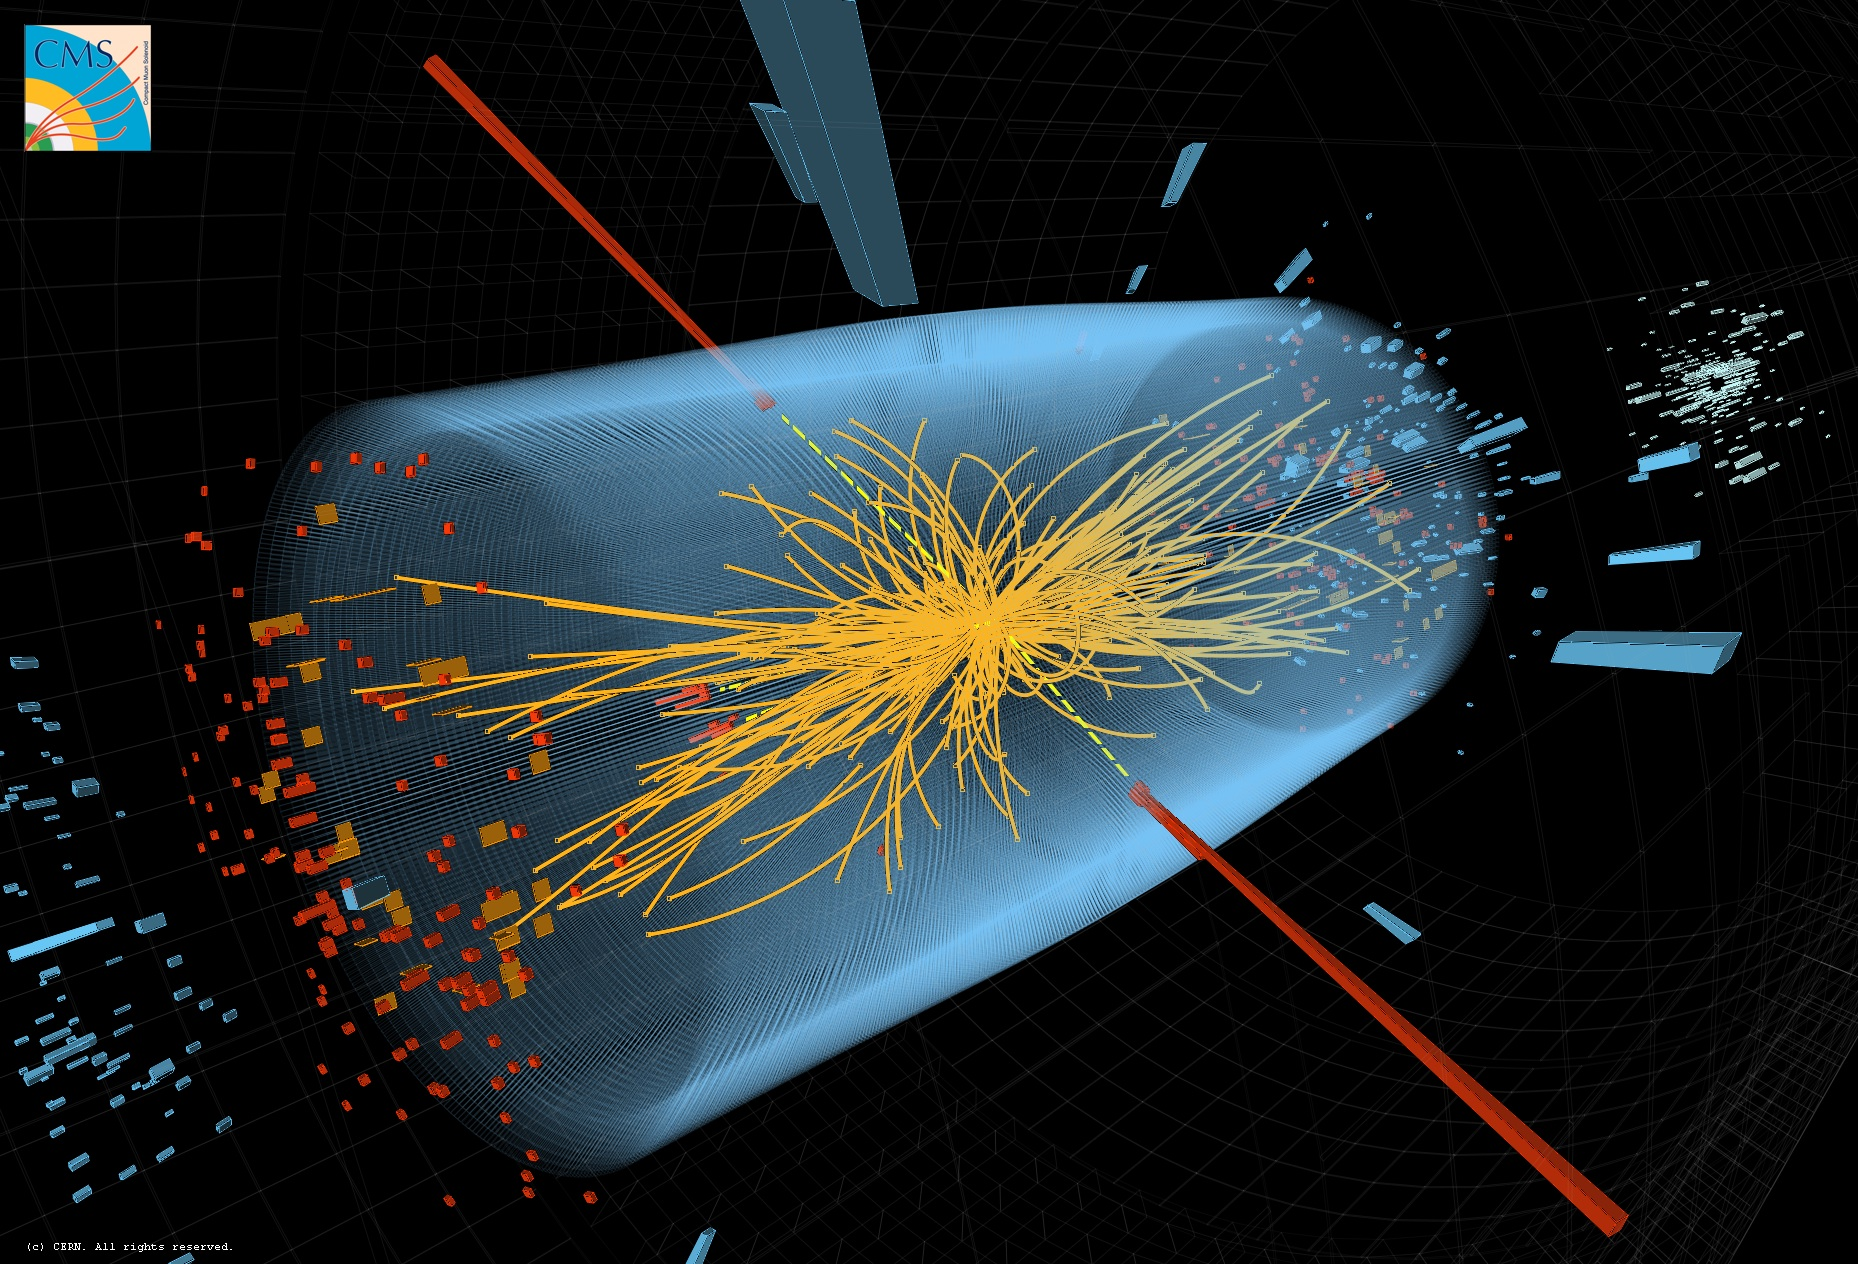
\includegraphics[width=0.6\textwidth]{figures/cms.jpg}
\end{frame}

\end{document}

